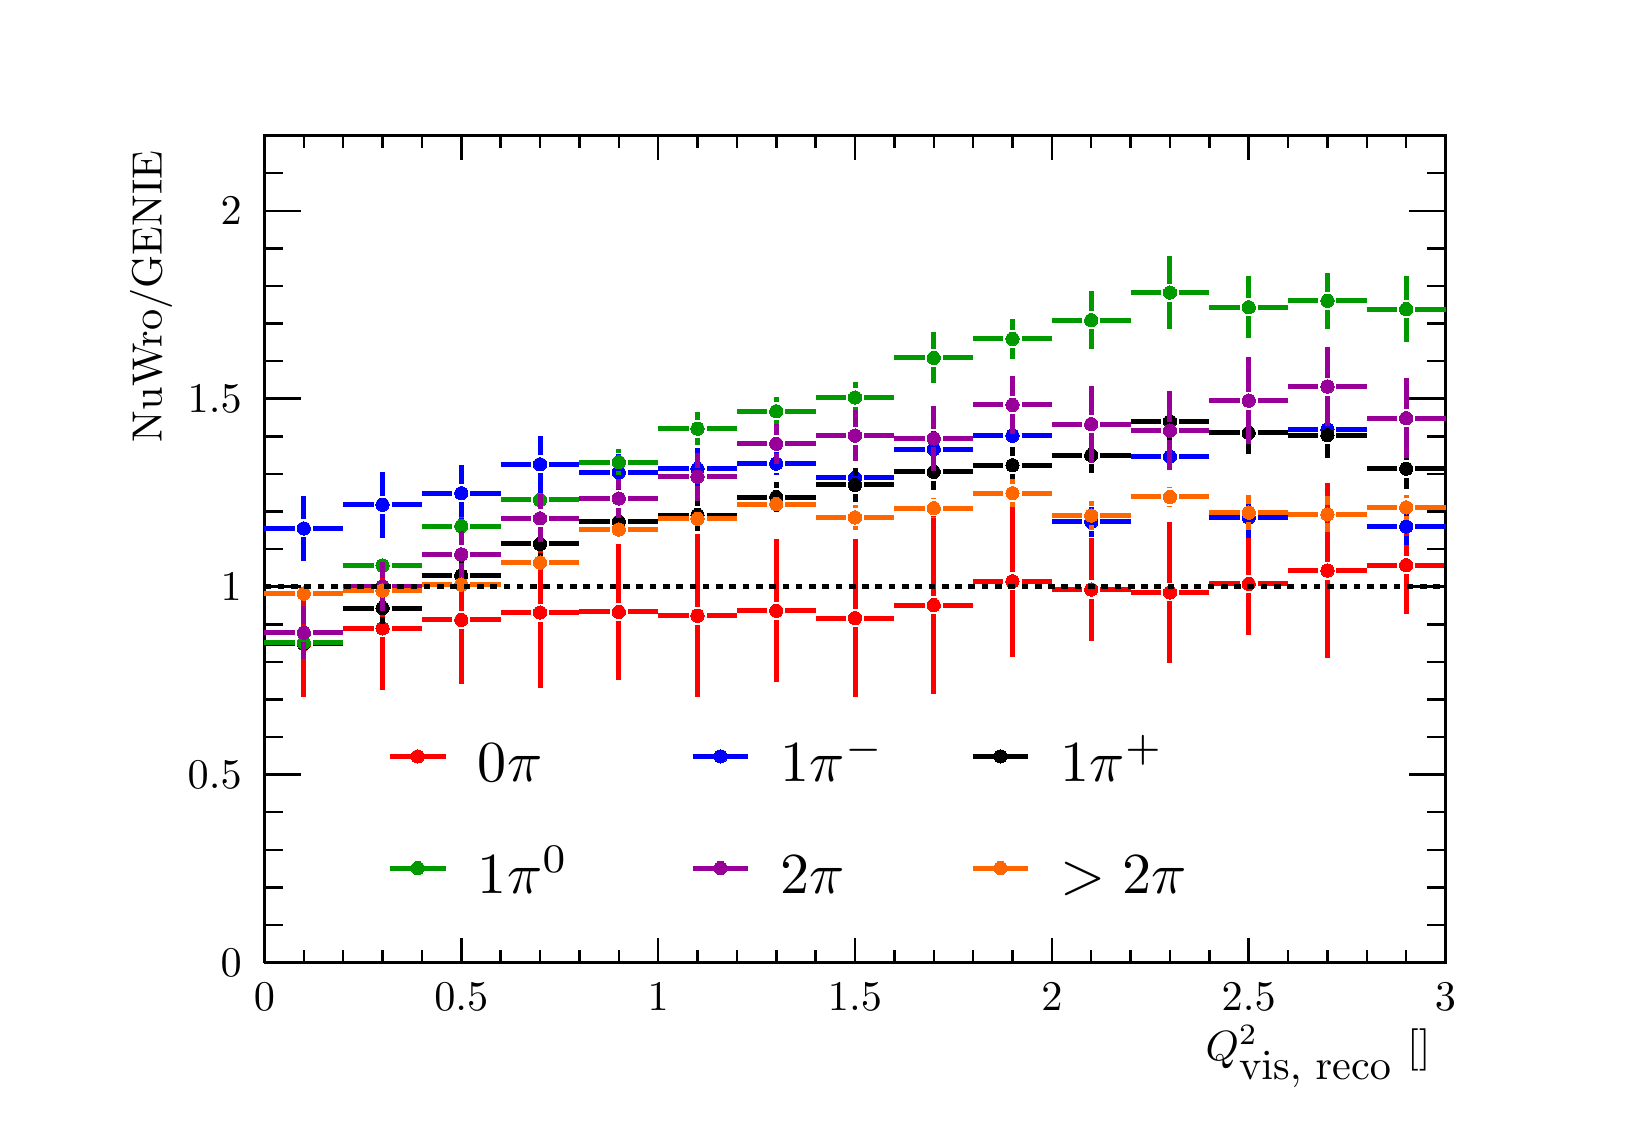
\begin{tikzpicture}
\pgfdeclareplotmark{cross} {
\pgfpathmoveto{\pgfpoint{-0.3\pgfplotmarksize}{\pgfplotmarksize}}
\pgfpathlineto{\pgfpoint{+0.3\pgfplotmarksize}{\pgfplotmarksize}}
\pgfpathlineto{\pgfpoint{+0.3\pgfplotmarksize}{0.3\pgfplotmarksize}}
\pgfpathlineto{\pgfpoint{+1\pgfplotmarksize}{0.3\pgfplotmarksize}}
\pgfpathlineto{\pgfpoint{+1\pgfplotmarksize}{-0.3\pgfplotmarksize}}
\pgfpathlineto{\pgfpoint{+0.3\pgfplotmarksize}{-0.3\pgfplotmarksize}}
\pgfpathlineto{\pgfpoint{+0.3\pgfplotmarksize}{-1.\pgfplotmarksize}}
\pgfpathlineto{\pgfpoint{-0.3\pgfplotmarksize}{-1.\pgfplotmarksize}}
\pgfpathlineto{\pgfpoint{-0.3\pgfplotmarksize}{-0.3\pgfplotmarksize}}
\pgfpathlineto{\pgfpoint{-1.\pgfplotmarksize}{-0.3\pgfplotmarksize}}
\pgfpathlineto{\pgfpoint{-1.\pgfplotmarksize}{0.3\pgfplotmarksize}}
\pgfpathlineto{\pgfpoint{-0.3\pgfplotmarksize}{0.3\pgfplotmarksize}}
\pgfpathclose
\pgfusepathqstroke
}
\pgfdeclareplotmark{cross*} {
\pgfpathmoveto{\pgfpoint{-0.3\pgfplotmarksize}{\pgfplotmarksize}}
\pgfpathlineto{\pgfpoint{+0.3\pgfplotmarksize}{\pgfplotmarksize}}
\pgfpathlineto{\pgfpoint{+0.3\pgfplotmarksize}{0.3\pgfplotmarksize}}
\pgfpathlineto{\pgfpoint{+1\pgfplotmarksize}{0.3\pgfplotmarksize}}
\pgfpathlineto{\pgfpoint{+1\pgfplotmarksize}{-0.3\pgfplotmarksize}}
\pgfpathlineto{\pgfpoint{+0.3\pgfplotmarksize}{-0.3\pgfplotmarksize}}
\pgfpathlineto{\pgfpoint{+0.3\pgfplotmarksize}{-1.\pgfplotmarksize}}
\pgfpathlineto{\pgfpoint{-0.3\pgfplotmarksize}{-1.\pgfplotmarksize}}
\pgfpathlineto{\pgfpoint{-0.3\pgfplotmarksize}{-0.3\pgfplotmarksize}}
\pgfpathlineto{\pgfpoint{-1.\pgfplotmarksize}{-0.3\pgfplotmarksize}}
\pgfpathlineto{\pgfpoint{-1.\pgfplotmarksize}{0.3\pgfplotmarksize}}
\pgfpathlineto{\pgfpoint{-0.3\pgfplotmarksize}{0.3\pgfplotmarksize}}
\pgfpathclose
\pgfusepathqfillstroke
}
\pgfdeclareplotmark{newstar} {
\pgfpathmoveto{\pgfqpoint{0pt}{\pgfplotmarksize}}
\pgfpathlineto{\pgfqpointpolar{44}{0.5\pgfplotmarksize}}
\pgfpathlineto{\pgfqpointpolar{18}{\pgfplotmarksize}}
\pgfpathlineto{\pgfqpointpolar{-20}{0.5\pgfplotmarksize}}
\pgfpathlineto{\pgfqpointpolar{-54}{\pgfplotmarksize}}
\pgfpathlineto{\pgfqpointpolar{-90}{0.5\pgfplotmarksize}}
\pgfpathlineto{\pgfqpointpolar{234}{\pgfplotmarksize}}
\pgfpathlineto{\pgfqpointpolar{198}{0.5\pgfplotmarksize}}
\pgfpathlineto{\pgfqpointpolar{162}{\pgfplotmarksize}}
\pgfpathlineto{\pgfqpointpolar{134}{0.5\pgfplotmarksize}}
\pgfpathclose
\pgfusepathqstroke
}
\pgfdeclareplotmark{newstar*} {
\pgfpathmoveto{\pgfqpoint{0pt}{\pgfplotmarksize}}
\pgfpathlineto{\pgfqpointpolar{44}{0.5\pgfplotmarksize}}
\pgfpathlineto{\pgfqpointpolar{18}{\pgfplotmarksize}}
\pgfpathlineto{\pgfqpointpolar{-20}{0.5\pgfplotmarksize}}
\pgfpathlineto{\pgfqpointpolar{-54}{\pgfplotmarksize}}
\pgfpathlineto{\pgfqpointpolar{-90}{0.5\pgfplotmarksize}}
\pgfpathlineto{\pgfqpointpolar{234}{\pgfplotmarksize}}
\pgfpathlineto{\pgfqpointpolar{198}{0.5\pgfplotmarksize}}
\pgfpathlineto{\pgfqpointpolar{162}{\pgfplotmarksize}}
\pgfpathlineto{\pgfqpointpolar{134}{0.5\pgfplotmarksize}}
\pgfpathclose
\pgfusepathqfillstroke
}
\definecolor{c}{rgb}{1,1,1};
\draw [color=c, fill=c] (0,0) rectangle (20,13.639);
\draw [color=c, fill=c] (3,1.77307) rectangle (18,12.2751);
\definecolor{c}{rgb}{0,0,0};
\draw [c,line width=0.9] (3,1.77307) -- (3,12.2751) -- (18,12.2751) -- (18,1.77307) -- (3,1.77307);
\definecolor{c}{rgb}{1,1,1};
\draw [color=c, fill=c] (3,1.77307) rectangle (18,12.2751);
\definecolor{c}{rgb}{0,0,0};
\draw [c,line width=0.9] (3,1.77307) -- (3,12.2751) -- (18,12.2751) -- (18,1.77307) -- (3,1.77307);
\definecolor{c}{rgb}{1,0,0};
\draw [c,line width=1.8] (3.5,5.14661) -- (3.5,5.70617);
\draw [c,line width=1.8] (3.5,5.93539) -- (3.5,6.49495);
\draw [c,line width=1.8] (3,5.82078) -- (3.38539,5.82078);
\draw [c,line width=1.8] (3.61461,5.82078) -- (4,5.82078);
\foreach \P in {(3.5,5.82078)}{\draw[mark options={color=c,fill=c},mark size=2.402402pt, line width=0.000000pt, mark=*] plot coordinates {\P};}
\draw [c,line width=1.8] (4.5,5.22838) -- (4.5,5.90216);
\draw [c,line width=1.8] (4.5,6.13139) -- (4.5,6.80517);
\draw [c,line width=1.8] (4,6.01677) -- (4.38539,6.01677);
\draw [c,line width=1.8] (4.61461,6.01677) -- (5,6.01677);
\foreach \P in {(4.5,6.01677)}{\draw[mark options={color=c,fill=c},mark size=2.402402pt, line width=0.000000pt, mark=*] plot coordinates {\P};}
\draw [c,line width=1.8] (5.5,5.31134) -- (5.5,6.01023);
\draw [c,line width=1.8] (5.5,6.23946) -- (5.5,6.93836);
\draw [c,line width=1.8] (5,6.12485) -- (5.38539,6.12485);
\draw [c,line width=1.8] (5.61461,6.12485) -- (6,6.12485);
\foreach \P in {(5.5,6.12485)}{\draw[mark options={color=c,fill=c},mark size=2.402402pt, line width=0.000000pt, mark=*] plot coordinates {\P};}
\draw [c,line width=1.8] (6.5,5.26536) -- (6.5,6.10349);
\draw [c,line width=1.8] (6.5,6.33272) -- (6.5,7.17086);
\draw [c,line width=1.8] (6,6.21811) -- (6.38539,6.21811);
\draw [c,line width=1.8] (6.61461,6.21811) -- (7,6.21811);
\foreach \P in {(6.5,6.21811)}{\draw[mark options={color=c,fill=c},mark size=2.402402pt, line width=0.000000pt, mark=*] plot coordinates {\P};}
\draw [c,line width=1.8] (7.5,5.36765) -- (7.5,6.11078);
\draw [c,line width=1.8] (7.5,6.34001) -- (7.5,7.08315);
\draw [c,line width=1.8] (7,6.2254) -- (7.38539,6.2254);
\draw [c,line width=1.8] (7.61461,6.2254) -- (8,6.2254);
\foreach \P in {(7.5,6.2254)}{\draw[mark options={color=c,fill=c},mark size=2.402402pt, line width=0.000000pt, mark=*] plot coordinates {\P};}
\draw [c,line width=1.8] (8.5,5.14631) -- (8.5,6.06352);
\draw [c,line width=1.8] (8.5,6.29274) -- (8.5,7.20995);
\draw [c,line width=1.8] (8,6.17813) -- (8.38539,6.17813);
\draw [c,line width=1.8] (8.61461,6.17813) -- (9,6.17813);
\foreach \P in {(8.5,6.17813)}{\draw[mark options={color=c,fill=c},mark size=2.402402pt, line width=0.000000pt, mark=*] plot coordinates {\P};}
\draw [c,line width=1.8] (9.5,5.33253) -- (9.5,6.12666);
\draw [c,line width=1.8] (9.5,6.35589) -- (9.5,7.15002);
\draw [c,line width=1.8] (9,6.24128) -- (9.38539,6.24128);
\draw [c,line width=1.8] (9.61461,6.24128) -- (10,6.24128);
\foreach \P in {(9.5,6.24128)}{\draw[mark options={color=c,fill=c},mark size=2.402402pt, line width=0.000000pt, mark=*] plot coordinates {\P};}
\draw [c,line width=1.8] (10.5,5.14499) -- (10.5,6.03227);
\draw [c,line width=1.8] (10.5,6.26149) -- (10.5,7.14877);
\draw [c,line width=1.8] (10,6.14688) -- (10.3854,6.14688);
\draw [c,line width=1.8] (10.6146,6.14688) -- (11,6.14688);
\foreach \P in {(10.5,6.14688)}{\draw[mark options={color=c,fill=c},mark size=2.402402pt, line width=0.000000pt, mark=*] plot coordinates {\P};}
\draw [c,line width=1.8] (11.5,5.1861) -- (11.5,6.19834);
\draw [c,line width=1.8] (11.5,6.42756) -- (11.5,7.4398);
\draw [c,line width=1.8] (11,6.31295) -- (11.3854,6.31295);
\draw [c,line width=1.8] (11.6146,6.31295) -- (12,6.31295);
\foreach \P in {(11.5,6.31295)}{\draw[mark options={color=c,fill=c},mark size=2.402402pt, line width=0.000000pt, mark=*] plot coordinates {\P};}
\draw [c,line width=1.8] (12.5,5.6489) -- (12.5,6.50107);
\draw [c,line width=1.8] (12.5,6.73029) -- (12.5,7.58246);
\draw [c,line width=1.8] (12,6.61568) -- (12.3854,6.61568);
\draw [c,line width=1.8] (12.6146,6.61568) -- (13,6.61568);
\foreach \P in {(12.5,6.61568)}{\draw[mark options={color=c,fill=c},mark size=2.402402pt, line width=0.000000pt, mark=*] plot coordinates {\P};}
\draw [c,line width=1.8] (13.5,5.86222) -- (13.5,6.39595);
\draw [c,line width=1.8] (13.5,6.62518) -- (13.5,7.15891);
\draw [c,line width=1.8] (13,6.51056) -- (13.3854,6.51056);
\draw [c,line width=1.8] (13.6146,6.51056) -- (14,6.51056);
\foreach \P in {(13.5,6.51056)}{\draw[mark options={color=c,fill=c},mark size=2.402402pt, line width=0.000000pt, mark=*] plot coordinates {\P};}
\draw [c,line width=1.8] (14.5,5.58125) -- (14.5,6.35889);
\draw [c,line width=1.8] (14.5,6.58812) -- (14.5,7.36577);
\draw [c,line width=1.8] (14,6.47351) -- (14.3854,6.47351);
\draw [c,line width=1.8] (14.6146,6.47351) -- (15,6.47351);
\foreach \P in {(14.5,6.47351)}{\draw[mark options={color=c,fill=c},mark size=2.402402pt, line width=0.000000pt, mark=*] plot coordinates {\P};}
\draw [c,line width=1.8] (15.5,5.9363) -- (15.5,6.46694);
\draw [c,line width=1.8] (15.5,6.69617) -- (15.5,7.22681);
\draw [c,line width=1.8] (15,6.58155) -- (15.3854,6.58155);
\draw [c,line width=1.8] (15.6146,6.58155) -- (16,6.58155);
\foreach \P in {(15.5,6.58155)}{\draw[mark options={color=c,fill=c},mark size=2.402402pt, line width=0.000000pt, mark=*] plot coordinates {\P};}
\draw [c,line width=1.8] (16.5,5.64389) -- (16.5,6.63659);
\draw [c,line width=1.8] (16.5,6.86582) -- (16.5,7.85852);
\draw [c,line width=1.8] (16,6.75121) -- (16.3854,6.75121);
\draw [c,line width=1.8] (16.6146,6.75121) -- (17,6.75121);
\foreach \P in {(16.5,6.75121)}{\draw[mark options={color=c,fill=c},mark size=2.402402pt, line width=0.000000pt, mark=*] plot coordinates {\P};}
\draw [c,line width=1.8] (17.5,6.19362) -- (17.5,6.70515);
\draw [c,line width=1.8] (17.5,6.93437) -- (17.5,7.44591);
\draw [c,line width=1.8] (17,6.81976) -- (17.3854,6.81976);
\draw [c,line width=1.8] (17.6146,6.81976) -- (18,6.81976);
\foreach \P in {(17.5,6.81976)}{\draw[mark options={color=c,fill=c},mark size=2.402402pt, line width=0.000000pt, mark=*] plot coordinates {\P};}
\definecolor{c}{rgb}{0,0,0};
\draw [c,line width=0.9] (3,1.77307) -- (18,1.77307);
\draw [c,line width=0.9] (3,2.07994) -- (3,1.77307);
\draw [c,line width=0.9] (3.5,1.9265) -- (3.5,1.77307);
\draw [c,line width=0.9] (4,1.9265) -- (4,1.77307);
\draw [c,line width=0.9] (4.5,1.9265) -- (4.5,1.77307);
\draw [c,line width=0.9] (5,1.9265) -- (5,1.77307);
\draw [c,line width=0.9] (5.5,2.07994) -- (5.5,1.77307);
\draw [c,line width=0.9] (6,1.9265) -- (6,1.77307);
\draw [c,line width=0.9] (6.5,1.9265) -- (6.5,1.77307);
\draw [c,line width=0.9] (7,1.9265) -- (7,1.77307);
\draw [c,line width=0.9] (7.5,1.9265) -- (7.5,1.77307);
\draw [c,line width=0.9] (8,2.07994) -- (8,1.77307);
\draw [c,line width=0.9] (8.5,1.9265) -- (8.5,1.77307);
\draw [c,line width=0.9] (9,1.9265) -- (9,1.77307);
\draw [c,line width=0.9] (9.5,1.9265) -- (9.5,1.77307);
\draw [c,line width=0.9] (10,1.9265) -- (10,1.77307);
\draw [c,line width=0.9] (10.5,2.07994) -- (10.5,1.77307);
\draw [c,line width=0.9] (11,1.9265) -- (11,1.77307);
\draw [c,line width=0.9] (11.5,1.9265) -- (11.5,1.77307);
\draw [c,line width=0.9] (12,1.9265) -- (12,1.77307);
\draw [c,line width=0.9] (12.5,1.9265) -- (12.5,1.77307);
\draw [c,line width=0.9] (13,2.07994) -- (13,1.77307);
\draw [c,line width=0.9] (13.5,1.9265) -- (13.5,1.77307);
\draw [c,line width=0.9] (14,1.9265) -- (14,1.77307);
\draw [c,line width=0.9] (14.5,1.9265) -- (14.5,1.77307);
\draw [c,line width=0.9] (15,1.9265) -- (15,1.77307);
\draw [c,line width=0.9] (15.5,2.07994) -- (15.5,1.77307);
\draw [c,line width=0.9] (16,1.9265) -- (16,1.77307);
\draw [c,line width=0.9] (16.5,1.9265) -- (16.5,1.77307);
\draw [c,line width=0.9] (17,1.9265) -- (17,1.77307);
\draw [c,line width=0.9] (17.5,1.9265) -- (17.5,1.77307);
\draw [c,line width=0.9] (18,2.07994) -- (18,1.77307);
\draw [c,line width=0.9] (18,2.07994) -- (18,1.77307);
\draw [anchor=base] (3,1.15931) node[scale=1.52731, color=c, rotate=0]{0};
\draw [anchor=base] (5.5,1.15931) node[scale=1.52731, color=c, rotate=0]{0.5};
\draw [anchor=base] (8,1.15931) node[scale=1.52731, color=c, rotate=0]{1};
\draw [anchor=base] (10.5,1.15931) node[scale=1.52731, color=c, rotate=0]{1.5};
\draw [anchor=base] (13,1.15931) node[scale=1.52731, color=c, rotate=0]{2};
\draw [anchor=base] (15.5,1.15931) node[scale=1.52731, color=c, rotate=0]{2.5};
\draw [anchor=base] (18,1.15931) node[scale=1.52731, color=c, rotate=0]{3};
\draw [anchor= east] (18,0.572837) node[scale=1.52731, color=c, rotate=0]{$Q^{2}_{\textrm{vis, reco}}$ [\si{\giga\electronvolt\squared}] };
\draw [c,line width=0.9] (3,12.2751) -- (18,12.2751);
\draw [c,line width=0.9] (3,11.9682) -- (3,12.2751);
\draw [c,line width=0.9] (3.5,12.1216) -- (3.5,12.2751);
\draw [c,line width=0.9] (4,12.1216) -- (4,12.2751);
\draw [c,line width=0.9] (4.5,12.1216) -- (4.5,12.2751);
\draw [c,line width=0.9] (5,12.1216) -- (5,12.2751);
\draw [c,line width=0.9] (5.5,11.9682) -- (5.5,12.2751);
\draw [c,line width=0.9] (6,12.1216) -- (6,12.2751);
\draw [c,line width=0.9] (6.5,12.1216) -- (6.5,12.2751);
\draw [c,line width=0.9] (7,12.1216) -- (7,12.2751);
\draw [c,line width=0.9] (7.5,12.1216) -- (7.5,12.2751);
\draw [c,line width=0.9] (8,11.9682) -- (8,12.2751);
\draw [c,line width=0.9] (8.5,12.1216) -- (8.5,12.2751);
\draw [c,line width=0.9] (9,12.1216) -- (9,12.2751);
\draw [c,line width=0.9] (9.5,12.1216) -- (9.5,12.2751);
\draw [c,line width=0.9] (10,12.1216) -- (10,12.2751);
\draw [c,line width=0.9] (10.5,11.9682) -- (10.5,12.2751);
\draw [c,line width=0.9] (11,12.1216) -- (11,12.2751);
\draw [c,line width=0.9] (11.5,12.1216) -- (11.5,12.2751);
\draw [c,line width=0.9] (12,12.1216) -- (12,12.2751);
\draw [c,line width=0.9] (12.5,12.1216) -- (12.5,12.2751);
\draw [c,line width=0.9] (13,11.9682) -- (13,12.2751);
\draw [c,line width=0.9] (13.5,12.1216) -- (13.5,12.2751);
\draw [c,line width=0.9] (14,12.1216) -- (14,12.2751);
\draw [c,line width=0.9] (14.5,12.1216) -- (14.5,12.2751);
\draw [c,line width=0.9] (15,12.1216) -- (15,12.2751);
\draw [c,line width=0.9] (15.5,11.9682) -- (15.5,12.2751);
\draw [c,line width=0.9] (16,12.1216) -- (16,12.2751);
\draw [c,line width=0.9] (16.5,12.1216) -- (16.5,12.2751);
\draw [c,line width=0.9] (17,12.1216) -- (17,12.2751);
\draw [c,line width=0.9] (17.5,12.1216) -- (17.5,12.2751);
\draw [c,line width=0.9] (18,11.9682) -- (18,12.2751);
\draw [c,line width=0.9] (18,11.9682) -- (18,12.2751);
\draw [c,line width=0.9] (3,1.77307) -- (3,12.2751);
\draw [c,line width=0.9] (3.462,1.77307) -- (3,1.77307);
\draw [c,line width=0.9] (3.231,2.25043) -- (3,2.25043);
\draw [c,line width=0.9] (3.231,2.72779) -- (3,2.72779);
\draw [c,line width=0.9] (3.231,3.20516) -- (3,3.20516);
\draw [c,line width=0.9] (3.231,3.68252) -- (3,3.68252);
\draw [c,line width=0.9] (3.462,4.15989) -- (3,4.15989);
\draw [c,line width=0.9] (3.231,4.63725) -- (3,4.63725);
\draw [c,line width=0.9] (3.231,5.11461) -- (3,5.11461);
\draw [c,line width=0.9] (3.231,5.59198) -- (3,5.59198);
\draw [c,line width=0.9] (3.231,6.06934) -- (3,6.06934);
\draw [c,line width=0.9] (3.462,6.5467) -- (3,6.5467);
\draw [c,line width=0.9] (3.231,7.02407) -- (3,7.02407);
\draw [c,line width=0.9] (3.231,7.50143) -- (3,7.50143);
\draw [c,line width=0.9] (3.231,7.9788) -- (3,7.9788);
\draw [c,line width=0.9] (3.231,8.45616) -- (3,8.45616);
\draw [c,line width=0.9] (3.462,8.93352) -- (3,8.93352);
\draw [c,line width=0.9] (3.231,9.41089) -- (3,9.41089);
\draw [c,line width=0.9] (3.231,9.88825) -- (3,9.88825);
\draw [c,line width=0.9] (3.231,10.3656) -- (3,10.3656);
\draw [c,line width=0.9] (3.231,10.843) -- (3,10.843);
\draw [c,line width=0.9] (3.462,11.3203) -- (3,11.3203);
\draw [c,line width=0.9] (3.462,11.3203) -- (3,11.3203);
\draw [c,line width=0.9] (3.231,11.7977) -- (3,11.7977);
\draw [c,line width=0.9] (3.231,12.2751) -- (3,12.2751);
\draw [anchor= east] (2.9,1.77307) node[scale=1.52731, color=c, rotate=0]{0};
\draw [anchor= east] (2.9,4.15989) node[scale=1.52731, color=c, rotate=0]{0.5};
\draw [anchor= east] (2.9,6.5467) node[scale=1.52731, color=c, rotate=0]{1};
\draw [anchor= east] (2.9,8.93352) node[scale=1.52731, color=c, rotate=0]{1.5};
\draw [anchor= east] (2.9,11.3203) node[scale=1.52731, color=c, rotate=0]{2};
\draw [anchor= east] (1.56,12.2751) node[scale=1.52731, color=c, rotate=90]{ NuWro/GENIE};
\draw [c,line width=0.9] (18,1.77307) -- (18,12.2751);
\draw [c,line width=0.9] (17.538,1.77307) -- (18,1.77307);
\draw [c,line width=0.9] (17.769,2.25043) -- (18,2.25043);
\draw [c,line width=0.9] (17.769,2.72779) -- (18,2.72779);
\draw [c,line width=0.9] (17.769,3.20516) -- (18,3.20516);
\draw [c,line width=0.9] (17.769,3.68252) -- (18,3.68252);
\draw [c,line width=0.9] (17.538,4.15989) -- (18,4.15989);
\draw [c,line width=0.9] (17.769,4.63725) -- (18,4.63725);
\draw [c,line width=0.9] (17.769,5.11461) -- (18,5.11461);
\draw [c,line width=0.9] (17.769,5.59198) -- (18,5.59198);
\draw [c,line width=0.9] (17.769,6.06934) -- (18,6.06934);
\draw [c,line width=0.9] (17.538,6.5467) -- (18,6.5467);
\draw [c,line width=0.9] (17.769,7.02407) -- (18,7.02407);
\draw [c,line width=0.9] (17.769,7.50143) -- (18,7.50143);
\draw [c,line width=0.9] (17.769,7.9788) -- (18,7.9788);
\draw [c,line width=0.9] (17.769,8.45616) -- (18,8.45616);
\draw [c,line width=0.9] (17.538,8.93352) -- (18,8.93352);
\draw [c,line width=0.9] (17.769,9.41089) -- (18,9.41089);
\draw [c,line width=0.9] (17.769,9.88825) -- (18,9.88825);
\draw [c,line width=0.9] (17.769,10.3656) -- (18,10.3656);
\draw [c,line width=0.9] (17.769,10.843) -- (18,10.843);
\draw [c,line width=0.9] (17.538,11.3203) -- (18,11.3203);
\draw [c,line width=0.9] (17.538,11.3203) -- (18,11.3203);
\draw [c,line width=0.9] (17.769,11.7977) -- (18,11.7977);
\draw [c,line width=0.9] (17.769,12.2751) -- (18,12.2751);
\definecolor{c}{rgb}{0,0,1};
\draw [c,line width=1.8] (3.5,6.87258) -- (3.5,7.17172);
\draw [c,line width=1.8] (3.5,7.40094) -- (3.5,7.70008);
\draw [c,line width=1.8] (3,7.28633) -- (3.38539,7.28633);
\draw [c,line width=1.8] (3.61461,7.28633) -- (4,7.28633);
\foreach \P in {(3.5,7.28633)}{\draw[mark options={color=c,fill=c},mark size=2.402402pt, line width=0.000000pt, mark=*] plot coordinates {\P};}
\draw [c,line width=1.8] (4.5,7.16978) -- (4.5,7.47235);
\draw [c,line width=1.8] (4.5,7.70157) -- (4.5,8.00414);
\draw [c,line width=1.8] (4,7.58696) -- (4.38539,7.58696);
\draw [c,line width=1.8] (4.61461,7.58696) -- (5,7.58696);
\foreach \P in {(4.5,7.58696)}{\draw[mark options={color=c,fill=c},mark size=2.402402pt, line width=0.000000pt, mark=*] plot coordinates {\P};}
\draw [c,line width=1.8] (5.5,7.36873) -- (5.5,7.61876);
\draw [c,line width=1.8] (5.5,7.84798) -- (5.5,8.09801);
\draw [c,line width=1.8] (5,7.73337) -- (5.38539,7.73337);
\draw [c,line width=1.8] (5.61461,7.73337) -- (6,7.73337);
\foreach \P in {(5.5,7.73337)}{\draw[mark options={color=c,fill=c},mark size=2.402402pt, line width=0.000000pt, mark=*] plot coordinates {\P};}
\draw [c,line width=1.8] (6.5,7.74061) -- (6.5,7.9861);
\draw [c,line width=1.8] (6.5,8.21533) -- (6.5,8.46083);
\draw [c,line width=1.8] (6,8.10072) -- (6.38539,8.10072);
\draw [c,line width=1.8] (6.61461,8.10072) -- (7,8.10072);
\foreach \P in {(6.5,8.10072)}{\draw[mark options={color=c,fill=c},mark size=2.402402pt, line width=0.000000pt, mark=*] plot coordinates {\P};}
\draw [c,line width=1.8] (7.5,7.76998) -- (7.5,7.88306);
\draw [c,line width=1.8] (7.5,8.11228) -- (7.5,8.22536);
\draw [c,line width=1.8] (7,7.99767) -- (7.38539,7.99767);
\draw [c,line width=1.8] (7.61461,7.99767) -- (8,7.99767);
\foreach \P in {(7.5,7.99767)}{\draw[mark options={color=c,fill=c},mark size=2.402402pt, line width=0.000000pt, mark=*] plot coordinates {\P};}
\draw [c,line width=1.8] (8.5,7.77122) -- (8.5,7.92789);
\draw [c,line width=1.8] (8.5,8.15712) -- (8.5,8.31379);
\draw [c,line width=1.8] (8,8.0425) -- (8.38539,8.0425);
\draw [c,line width=1.8] (8.61461,8.0425) -- (9,8.0425);
\foreach \P in {(8.5,8.0425)}{\draw[mark options={color=c,fill=c},mark size=2.402402pt, line width=0.000000pt, mark=*] plot coordinates {\P};}
\draw [c,line width=1.8] (9.5,7.95857) -- (9.5,7.99473);
\draw [c,line width=1.8] (9.5,8.22395) -- (9.5,8.26011);
\draw [c,line width=1.8] (9,8.10934) -- (9.38539,8.10934);
\draw [c,line width=1.8] (9.61461,8.10934) -- (10,8.10934);
\foreach \P in {(9.5,8.10934)}{\draw[mark options={color=c,fill=c},mark size=2.402402pt, line width=0.000000pt, mark=*] plot coordinates {\P};}
\draw [c,line width=1.8] (10.5,7.79799) -- (10.5,7.81246);
\draw [c,line width=1.8] (10.5,8.04168) -- (10.5,8.05615);
\draw [c,line width=1.8] (10,7.92707) -- (10.3854,7.92707);
\draw [c,line width=1.8] (10.6146,7.92707) -- (11,7.92707);
\foreach \P in {(10.5,7.92707)}{\draw[mark options={color=c,fill=c},mark size=2.402402pt, line width=0.000000pt, mark=*] plot coordinates {\P};}
\draw [c,line width=1.8] (11.5,8.05913) -- (11.5,8.17948);
\draw [c,line width=1.8] (11.5,8.40871) -- (11.5,8.52906);
\draw [c,line width=1.8] (11,8.2941) -- (11.3854,8.2941);
\draw [c,line width=1.8] (11.6146,8.2941) -- (12,8.2941);
\foreach \P in {(11.5,8.2941)}{\draw[mark options={color=c,fill=c},mark size=2.402402pt, line width=0.000000pt, mark=*] plot coordinates {\P};}
\draw [c,line width=1.8] (12,8.46437) -- (12.3854,8.46437);
\draw [c,line width=1.8] (12.6146,8.46437) -- (13,8.46437);
\foreach \P in {(12.5,8.46437)}{\draw[mark options={color=c,fill=c},mark size=2.402402pt, line width=0.000000pt, mark=*] plot coordinates {\P};}
\draw [c,line width=1.8] (13.5,7.17951) -- (13.5,7.25454);
\draw [c,line width=1.8] (13.5,7.48376) -- (13.5,7.55879);
\draw [c,line width=1.8] (13,7.36915) -- (13.3854,7.36915);
\draw [c,line width=1.8] (13.6146,7.36915) -- (14,7.36915);
\foreach \P in {(13.5,7.36915)}{\draw[mark options={color=c,fill=c},mark size=2.402402pt, line width=0.000000pt, mark=*] plot coordinates {\P};}
\draw [c,line width=1.8] (14.5,8.05396) -- (14.5,8.0838);
\draw [c,line width=1.8] (14.5,8.31303) -- (14.5,8.34286);
\draw [c,line width=1.8] (14,8.19841) -- (14.3854,8.19841);
\draw [c,line width=1.8] (14.6146,8.19841) -- (15,8.19841);
\foreach \P in {(14.5,8.19841)}{\draw[mark options={color=c,fill=c},mark size=2.402402pt, line width=0.000000pt, mark=*] plot coordinates {\P};}
\draw [c,line width=1.8] (15.5,7.16613) -- (15.5,7.31003);
\draw [c,line width=1.8] (15.5,7.53926) -- (15.5,7.68316);
\draw [c,line width=1.8] (15,7.42465) -- (15.3854,7.42465);
\draw [c,line width=1.8] (15.6146,7.42465) -- (16,7.42465);
\foreach \P in {(15.5,7.42465)}{\draw[mark options={color=c,fill=c},mark size=2.402402pt, line width=0.000000pt, mark=*] plot coordinates {\P};}
\draw [c,line width=1.8] (16,8.54401) -- (16.3854,8.54401);
\draw [c,line width=1.8] (16.6146,8.54401) -- (17,8.54401);
\foreach \P in {(16.5,8.54401)}{\draw[mark options={color=c,fill=c},mark size=2.402402pt, line width=0.000000pt, mark=*] plot coordinates {\P};}
\draw [c,line width=1.8] (17.5,7.08202) -- (17.5,7.19622);
\draw [c,line width=1.8] (17.5,7.42545) -- (17.5,7.53965);
\draw [c,line width=1.8] (17,7.31084) -- (17.3854,7.31084);
\draw [c,line width=1.8] (17.6146,7.31084) -- (18,7.31084);
\foreach \P in {(17.5,7.31084)}{\draw[mark options={color=c,fill=c},mark size=2.402402pt, line width=0.000000pt, mark=*] plot coordinates {\P};}
\definecolor{c}{rgb}{0,0,0};
\draw [c,line width=1.8] (3.5,5.6285) -- (3.5,5.70878);
\draw [c,line width=1.8] (3.5,5.938) -- (3.5,6.01828);
\draw [c,line width=1.8] (3,5.82339) -- (3.38539,5.82339);
\draw [c,line width=1.8] (3.61461,5.82339) -- (4,5.82339);
\foreach \P in {(3.5,5.82339)}{\draw[mark options={color=c,fill=c},mark size=2.402402pt, line width=0.000000pt, mark=*] plot coordinates {\P};}
\draw [c,line width=1.8] (4.5,6.07069) -- (4.5,6.16101);
\draw [c,line width=1.8] (4.5,6.39023) -- (4.5,6.48056);
\draw [c,line width=1.8] (4,6.27562) -- (4.38539,6.27562);
\draw [c,line width=1.8] (4.61461,6.27562) -- (5,6.27562);
\foreach \P in {(4.5,6.27562)}{\draw[mark options={color=c,fill=c},mark size=2.402402pt, line width=0.000000pt, mark=*] plot coordinates {\P};}
\draw [c,line width=1.8] (5.5,6.49851) -- (5.5,6.5715);
\draw [c,line width=1.8] (5.5,6.80073) -- (5.5,6.87372);
\draw [c,line width=1.8] (5,6.68612) -- (5.38539,6.68612);
\draw [c,line width=1.8] (5.61461,6.68612) -- (6,6.68612);
\foreach \P in {(5.5,6.68612)}{\draw[mark options={color=c,fill=c},mark size=2.402402pt, line width=0.000000pt, mark=*] plot coordinates {\P};}
\draw [c,line width=1.8] (6.5,6.88677) -- (6.5,6.97418);
\draw [c,line width=1.8] (6.5,7.20341) -- (6.5,7.29082);
\draw [c,line width=1.8] (6,7.08879) -- (6.38539,7.08879);
\draw [c,line width=1.8] (6.61461,7.08879) -- (7,7.08879);
\foreach \P in {(6.5,7.08879)}{\draw[mark options={color=c,fill=c},mark size=2.402402pt, line width=0.000000pt, mark=*] plot coordinates {\P};}
\draw [c,line width=1.8] (7.5,7.20297) -- (7.5,7.25703);
\draw [c,line width=1.8] (7.5,7.48626) -- (7.5,7.54032);
\draw [c,line width=1.8] (7,7.37164) -- (7.38539,7.37164);
\draw [c,line width=1.8] (7.61461,7.37164) -- (8,7.37164);
\foreach \P in {(7.5,7.37164)}{\draw[mark options={color=c,fill=c},mark size=2.402402pt, line width=0.000000pt, mark=*] plot coordinates {\P};}
\draw [c,line width=1.8] (8.5,7.25065) -- (8.5,7.34104);
\draw [c,line width=1.8] (8.5,7.57027) -- (8.5,7.66066);
\draw [c,line width=1.8] (8,7.45566) -- (8.38539,7.45566);
\draw [c,line width=1.8] (8.61461,7.45566) -- (9,7.45566);
\foreach \P in {(8.5,7.45566)}{\draw[mark options={color=c,fill=c},mark size=2.402402pt, line width=0.000000pt, mark=*] plot coordinates {\P};}
\draw [c,line width=1.8] (9.5,7.49448) -- (9.5,7.57027);
\draw [c,line width=1.8] (9.5,7.7995) -- (9.5,7.87529);
\draw [c,line width=1.8] (9,7.68488) -- (9.38539,7.68488);
\draw [c,line width=1.8] (9.61461,7.68488) -- (10,7.68488);
\foreach \P in {(9.5,7.68488)}{\draw[mark options={color=c,fill=c},mark size=2.402402pt, line width=0.000000pt, mark=*] plot coordinates {\P};}
\draw [c,line width=1.8] (10.5,7.62831) -- (10.5,7.72538);
\draw [c,line width=1.8] (10.5,7.9546) -- (10.5,8.05167);
\draw [c,line width=1.8] (10,7.83999) -- (10.3854,7.83999);
\draw [c,line width=1.8] (10.6146,7.83999) -- (11,7.83999);
\foreach \P in {(10.5,7.83999)}{\draw[mark options={color=c,fill=c},mark size=2.402402pt, line width=0.000000pt, mark=*] plot coordinates {\P};}
\draw [c,line width=1.8] (11.5,7.78061) -- (11.5,7.88934);
\draw [c,line width=1.8] (11.5,8.11857) -- (11.5,8.22731);
\draw [c,line width=1.8] (11,8.00396) -- (11.3854,8.00396);
\draw [c,line width=1.8] (11.6146,8.00396) -- (12,8.00396);
\foreach \P in {(11.5,8.00396)}{\draw[mark options={color=c,fill=c},mark size=2.402402pt, line width=0.000000pt, mark=*] plot coordinates {\P};}
\draw [c,line width=1.8] (12.5,7.85813) -- (12.5,7.97461);
\draw [c,line width=1.8] (12.5,8.20383) -- (12.5,8.32031);
\draw [c,line width=1.8] (12,8.08922) -- (12.3854,8.08922);
\draw [c,line width=1.8] (12.6146,8.08922) -- (13,8.08922);
\foreach \P in {(12.5,8.08922)}{\draw[mark options={color=c,fill=c},mark size=2.402402pt, line width=0.000000pt, mark=*] plot coordinates {\P};}
\draw [c,line width=1.8] (13.5,7.99116) -- (13.5,8.10285);
\draw [c,line width=1.8] (13.5,8.33208) -- (13.5,8.44376);
\draw [c,line width=1.8] (13,8.21746) -- (13.3854,8.21746);
\draw [c,line width=1.8] (13.6146,8.21746) -- (14,8.21746);
\foreach \P in {(13.5,8.21746)}{\draw[mark options={color=c,fill=c},mark size=2.402402pt, line width=0.000000pt, mark=*] plot coordinates {\P};}
\draw [c,line width=1.8] (14.5,8.32529) -- (14.5,8.53043);
\draw [c,line width=1.8] (14.5,8.75965) -- (14.5,8.96478);
\draw [c,line width=1.8] (14,8.64504) -- (14.3854,8.64504);
\draw [c,line width=1.8] (14.6146,8.64504) -- (15,8.64504);
\foreach \P in {(14.5,8.64504)}{\draw[mark options={color=c,fill=c},mark size=2.402402pt, line width=0.000000pt, mark=*] plot coordinates {\P};}
\draw [c,line width=1.8] (15.5,8.23443) -- (15.5,8.38441);
\draw [c,line width=1.8] (15.5,8.61363) -- (15.5,8.76361);
\draw [c,line width=1.8] (15,8.49902) -- (15.3854,8.49902);
\draw [c,line width=1.8] (15.6146,8.49902) -- (16,8.49902);
\foreach \P in {(15.5,8.49902)}{\draw[mark options={color=c,fill=c},mark size=2.402402pt, line width=0.000000pt, mark=*] plot coordinates {\P};}
\draw [c,line width=1.8] (16.5,8.1857) -- (16.5,8.35583);
\draw [c,line width=1.8] (16.5,8.58506) -- (16.5,8.75518);
\draw [c,line width=1.8] (16,8.47044) -- (16.3854,8.47044);
\draw [c,line width=1.8] (16.6146,8.47044) -- (17,8.47044);
\foreach \P in {(16.5,8.47044)}{\draw[mark options={color=c,fill=c},mark size=2.402402pt, line width=0.000000pt, mark=*] plot coordinates {\P};}
\draw [c,line width=1.8] (17.5,7.79178) -- (17.5,7.93035);
\draw [c,line width=1.8] (17.5,8.15958) -- (17.5,8.29815);
\draw [c,line width=1.8] (17,8.04496) -- (17.3854,8.04496);
\draw [c,line width=1.8] (17.6146,8.04496) -- (18,8.04496);
\foreach \P in {(17.5,8.04496)}{\draw[mark options={color=c,fill=c},mark size=2.402402pt, line width=0.000000pt, mark=*] plot coordinates {\P};}
\definecolor{c}{rgb}{0,0.6,0};
\draw [c,line width=1.8] (3,5.8352) -- (3.38539,5.8352);
\draw [c,line width=1.8] (3.61461,5.8352) -- (4,5.8352);
\foreach \P in {(3.5,5.8352)}{\draw[mark options={color=c,fill=c},mark size=2.402402pt, line width=0.000000pt, mark=*] plot coordinates {\P};}
\draw [c,line width=1.8] (4,6.81494) -- (4.38539,6.81494);
\draw [c,line width=1.8] (4.61461,6.81494) -- (5,6.81494);
\foreach \P in {(4.5,6.81494)}{\draw[mark options={color=c,fill=c},mark size=2.402402pt, line width=0.000000pt, mark=*] plot coordinates {\P};}
\draw [c,line width=1.8] (5.5,7.19657) -- (5.5,7.20161);
\draw [c,line width=1.8] (5.5,7.43084) -- (5.5,7.43587);
\draw [c,line width=1.8] (5,7.31622) -- (5.38539,7.31622);
\draw [c,line width=1.8] (5.61461,7.31622) -- (6,7.31622);
\foreach \P in {(5.5,7.31622)}{\draw[mark options={color=c,fill=c},mark size=2.402402pt, line width=0.000000pt, mark=*] plot coordinates {\P};}
\draw [c,line width=1.8] (6,7.64871) -- (6.38539,7.64871);
\draw [c,line width=1.8] (6.61461,7.64871) -- (7,7.64871);
\foreach \P in {(6.5,7.64871)}{\draw[mark options={color=c,fill=c},mark size=2.402402pt, line width=0.000000pt, mark=*] plot coordinates {\P};}
\draw [c,line width=1.8] (7.5,7.96273) -- (7.5,8.01349);
\draw [c,line width=1.8] (7.5,8.24271) -- (7.5,8.29348);
\draw [c,line width=1.8] (7,8.1281) -- (7.38539,8.1281);
\draw [c,line width=1.8] (7.61461,8.1281) -- (8,8.1281);
\foreach \P in {(7.5,8.1281)}{\draw[mark options={color=c,fill=c},mark size=2.402402pt, line width=0.000000pt, mark=*] plot coordinates {\P};}
\draw [c,line width=1.8] (8.5,8.34083) -- (8.5,8.43886);
\draw [c,line width=1.8] (8.5,8.66809) -- (8.5,8.76612);
\draw [c,line width=1.8] (8,8.55347) -- (8.38539,8.55347);
\draw [c,line width=1.8] (8.61461,8.55347) -- (9,8.55347);
\foreach \P in {(8.5,8.55347)}{\draw[mark options={color=c,fill=c},mark size=2.402402pt, line width=0.000000pt, mark=*] plot coordinates {\P};}
\draw [c,line width=1.8] (9.5,8.59098) -- (9.5,8.65888);
\draw [c,line width=1.8] (9.5,8.8881) -- (9.5,8.956);
\draw [c,line width=1.8] (9,8.77349) -- (9.38539,8.77349);
\draw [c,line width=1.8] (9.61461,8.77349) -- (10,8.77349);
\foreach \P in {(9.5,8.77349)}{\draw[mark options={color=c,fill=c},mark size=2.402402pt, line width=0.000000pt, mark=*] plot coordinates {\P};}
\draw [c,line width=1.8] (10.5,8.74843) -- (10.5,8.83433);
\draw [c,line width=1.8] (10.5,9.06356) -- (10.5,9.14947);
\draw [c,line width=1.8] (10,8.94895) -- (10.3854,8.94895);
\draw [c,line width=1.8] (10.6146,8.94895) -- (11,8.94895);
\foreach \P in {(10.5,8.94895)}{\draw[mark options={color=c,fill=c},mark size=2.402402pt, line width=0.000000pt, mark=*] plot coordinates {\P};}
\draw [c,line width=1.8] (11.5,9.12774) -- (11.5,9.33724);
\draw [c,line width=1.8] (11.5,9.56647) -- (11.5,9.77597);
\draw [c,line width=1.8] (11,9.45186) -- (11.3854,9.45186);
\draw [c,line width=1.8] (11.6146,9.45186) -- (12,9.45186);
\foreach \P in {(11.5,9.45186)}{\draw[mark options={color=c,fill=c},mark size=2.402402pt, line width=0.000000pt, mark=*] plot coordinates {\P};}
\draw [c,line width=1.8] (12.5,9.44176) -- (12.5,9.57887);
\draw [c,line width=1.8] (12.5,9.8081) -- (12.5,9.9452);
\draw [c,line width=1.8] (12,9.69349) -- (12.3854,9.69349);
\draw [c,line width=1.8] (12.6146,9.69349) -- (13,9.69349);
\foreach \P in {(12.5,9.69349)}{\draw[mark options={color=c,fill=c},mark size=2.402402pt, line width=0.000000pt, mark=*] plot coordinates {\P};}
\draw [c,line width=1.8] (13.5,9.56218) -- (13.5,9.81668);
\draw [c,line width=1.8] (13.5,10.0459) -- (13.5,10.3004);
\draw [c,line width=1.8] (13,9.93129) -- (13.3854,9.93129);
\draw [c,line width=1.8] (13.6146,9.93129) -- (14,9.93129);
\foreach \P in {(13.5,9.93129)}{\draw[mark options={color=c,fill=c},mark size=2.402402pt, line width=0.000000pt, mark=*] plot coordinates {\P};}
\draw [c,line width=1.8] (14.5,9.82351) -- (14.5,10.1673);
\draw [c,line width=1.8] (14.5,10.3965) -- (14.5,10.7403);
\draw [c,line width=1.8] (14,10.2819) -- (14.3854,10.2819);
\draw [c,line width=1.8] (14.6146,10.2819) -- (15,10.2819);
\foreach \P in {(14.5,10.2819)}{\draw[mark options={color=c,fill=c},mark size=2.402402pt, line width=0.000000pt, mark=*] plot coordinates {\P};}
\draw [c,line width=1.8] (15.5,9.69907) -- (15.5,9.98016);
\draw [c,line width=1.8] (15.5,10.2094) -- (15.5,10.4905);
\draw [c,line width=1.8] (15,10.0948) -- (15.3854,10.0948);
\draw [c,line width=1.8] (15.6146,10.0948) -- (16,10.0948);
\foreach \P in {(15.5,10.0948)}{\draw[mark options={color=c,fill=c},mark size=2.402402pt, line width=0.000000pt, mark=*] plot coordinates {\P};}
\draw [c,line width=1.8] (16.5,9.82222) -- (16.5,10.0627);
\draw [c,line width=1.8] (16.5,10.2919) -- (16.5,10.5323);
\draw [c,line width=1.8] (16,10.1773) -- (16.3854,10.1773);
\draw [c,line width=1.8] (16.6146,10.1773) -- (17,10.1773);
\foreach \P in {(16.5,10.1773)}{\draw[mark options={color=c,fill=c},mark size=2.402402pt, line width=0.000000pt, mark=*] plot coordinates {\P};}
\draw [c,line width=1.8] (17.5,9.65546) -- (17.5,9.95702);
\draw [c,line width=1.8] (17.5,10.1862) -- (17.5,10.4878);
\draw [c,line width=1.8] (17,10.0716) -- (17.3854,10.0716);
\draw [c,line width=1.8] (17.6146,10.0716) -- (18,10.0716);
\foreach \P in {(17.5,10.0716)}{\draw[mark options={color=c,fill=c},mark size=2.402402pt, line width=0.000000pt, mark=*] plot coordinates {\P};}
\definecolor{c}{rgb}{0.6,0,0.6};
\draw [c,line width=1.8] (3.5,5.62481) -- (3.5,5.84757);
\draw [c,line width=1.8] (3.5,6.0768) -- (3.5,6.29956);
\draw [c,line width=1.8] (3,5.96219) -- (3.38539,5.96219);
\draw [c,line width=1.8] (3.61461,5.96219) -- (4,5.96219);
\foreach \P in {(3.5,5.96219)}{\draw[mark options={color=c,fill=c},mark size=2.402402pt, line width=0.000000pt, mark=*] plot coordinates {\P};}
\draw [c,line width=1.8] (4.5,6.2336) -- (4.5,6.43368);
\draw [c,line width=1.8] (4.5,6.66291) -- (4.5,6.86298);
\draw [c,line width=1.8] (4,6.54829) -- (4.38539,6.54829);
\draw [c,line width=1.8] (4.61461,6.54829) -- (5,6.54829);
\foreach \P in {(4.5,6.54829)}{\draw[mark options={color=c,fill=c},mark size=2.402402pt, line width=0.000000pt, mark=*] plot coordinates {\P};}
\draw [c,line width=1.8] (5.5,6.66199) -- (5.5,6.84218);
\draw [c,line width=1.8] (5.5,7.07141) -- (5.5,7.25159);
\draw [c,line width=1.8] (5,6.95679) -- (5.38539,6.95679);
\draw [c,line width=1.8] (5.61461,6.95679) -- (6,6.95679);
\foreach \P in {(5.5,6.95679)}{\draw[mark options={color=c,fill=c},mark size=2.402402pt, line width=0.000000pt, mark=*] plot coordinates {\P};}
\draw [c,line width=1.8] (6.5,7.11113) -- (6.5,7.29975);
\draw [c,line width=1.8] (6.5,7.52898) -- (6.5,7.7176);
\draw [c,line width=1.8] (6,7.41436) -- (6.38539,7.41436);
\draw [c,line width=1.8] (6.61461,7.41436) -- (7,7.41436);
\foreach \P in {(6.5,7.41436)}{\draw[mark options={color=c,fill=c},mark size=2.402402pt, line width=0.000000pt, mark=*] plot coordinates {\P};}
\draw [c,line width=1.8] (7.5,7.41376) -- (7.5,7.55175);
\draw [c,line width=1.8] (7.5,7.78097) -- (7.5,7.91896);
\draw [c,line width=1.8] (7,7.66636) -- (7.38539,7.66636);
\draw [c,line width=1.8] (7.61461,7.66636) -- (8,7.66636);
\foreach \P in {(7.5,7.66636)}{\draw[mark options={color=c,fill=c},mark size=2.402402pt, line width=0.000000pt, mark=*] plot coordinates {\P};}
\draw [c,line width=1.8] (8.5,7.63799) -- (8.5,7.82923);
\draw [c,line width=1.8] (8.5,8.05845) -- (8.5,8.24969);
\draw [c,line width=1.8] (8,7.94384) -- (8.38539,7.94384);
\draw [c,line width=1.8] (8.61461,7.94384) -- (9,7.94384);
\foreach \P in {(8.5,7.94384)}{\draw[mark options={color=c,fill=c},mark size=2.402402pt, line width=0.000000pt, mark=*] plot coordinates {\P};}
\draw [c,line width=1.8] (9.5,8.10533) -- (9.5,8.24739);
\draw [c,line width=1.8] (9.5,8.47662) -- (9.5,8.61868);
\draw [c,line width=1.8] (9,8.36201) -- (9.38539,8.36201);
\draw [c,line width=1.8] (9.61461,8.36201) -- (10,8.36201);
\foreach \P in {(9.5,8.36201)}{\draw[mark options={color=c,fill=c},mark size=2.402402pt, line width=0.000000pt, mark=*] plot coordinates {\P};}
\draw [c,line width=1.8] (10.5,8.14331) -- (10.5,8.35096);
\draw [c,line width=1.8] (10.5,8.58019) -- (10.5,8.78784);
\draw [c,line width=1.8] (10,8.46558) -- (10.3854,8.46558);
\draw [c,line width=1.8] (10.6146,8.46558) -- (11,8.46558);
\foreach \P in {(10.5,8.46558)}{\draw[mark options={color=c,fill=c},mark size=2.402402pt, line width=0.000000pt, mark=*] plot coordinates {\P};}
\draw [c,line width=1.8] (11.5,8.01742) -- (11.5,8.31414);
\draw [c,line width=1.8] (11.5,8.54336) -- (11.5,8.84008);
\draw [c,line width=1.8] (11,8.42875) -- (11.3854,8.42875);
\draw [c,line width=1.8] (11.6146,8.42875) -- (12,8.42875);
\foreach \P in {(11.5,8.42875)}{\draw[mark options={color=c,fill=c},mark size=2.402402pt, line width=0.000000pt, mark=*] plot coordinates {\P};}
\draw [c,line width=1.8] (12.5,8.48727) -- (12.5,8.73973);
\draw [c,line width=1.8] (12.5,8.96896) -- (12.5,9.22142);
\draw [c,line width=1.8] (12,8.85435) -- (12.3854,8.85435);
\draw [c,line width=1.8] (12.6146,8.85435) -- (13,8.85435);
\foreach \P in {(12.5,8.85435)}{\draw[mark options={color=c,fill=c},mark size=2.402402pt, line width=0.000000pt, mark=*] plot coordinates {\P};}
\draw [c,line width=1.8] (13.5,8.12245) -- (13.5,8.49621);
\draw [c,line width=1.8] (13.5,8.72544) -- (13.5,9.0992);
\draw [c,line width=1.8] (13,8.61083) -- (13.3854,8.61083);
\draw [c,line width=1.8] (13.6146,8.61083) -- (14,8.61083);
\foreach \P in {(13.5,8.61083)}{\draw[mark options={color=c,fill=c},mark size=2.402402pt, line width=0.000000pt, mark=*] plot coordinates {\P};}
\draw [c,line width=1.8] (14.5,8.02351) -- (14.5,8.41424);
\draw [c,line width=1.8] (14.5,8.64347) -- (14.5,9.0342);
\draw [c,line width=1.8] (14,8.52886) -- (14.3854,8.52886);
\draw [c,line width=1.8] (14.6146,8.52886) -- (15,8.52886);
\foreach \P in {(14.5,8.52886)}{\draw[mark options={color=c,fill=c},mark size=2.402402pt, line width=0.000000pt, mark=*] plot coordinates {\P};}
\draw [c,line width=1.8] (15.5,8.35742) -- (15.5,8.7946);
\draw [c,line width=1.8] (15.5,9.02383) -- (15.5,9.46101);
\draw [c,line width=1.8] (15,8.90921) -- (15.3854,8.90921);
\draw [c,line width=1.8] (15.6146,8.90921) -- (16,8.90921);
\foreach \P in {(15.5,8.90921)}{\draw[mark options={color=c,fill=c},mark size=2.402402pt, line width=0.000000pt, mark=*] plot coordinates {\P};}
\draw [c,line width=1.8] (16.5,8.59099) -- (16.5,8.97312);
\draw [c,line width=1.8] (16.5,9.20234) -- (16.5,9.58447);
\draw [c,line width=1.8] (16,9.08773) -- (16.3854,9.08773);
\draw [c,line width=1.8] (16.6146,9.08773) -- (17,9.08773);
\foreach \P in {(16.5,9.08773)}{\draw[mark options={color=c,fill=c},mark size=2.402402pt, line width=0.000000pt, mark=*] plot coordinates {\P};}
\draw [c,line width=1.8] (17.5,8.17702) -- (17.5,8.57187);
\draw [c,line width=1.8] (17.5,8.80109) -- (17.5,9.19594);
\draw [c,line width=1.8] (17,8.68648) -- (17.3854,8.68648);
\draw [c,line width=1.8] (17.6146,8.68648) -- (18,8.68648);
\foreach \P in {(17.5,8.68648)}{\draw[mark options={color=c,fill=c},mark size=2.402402pt, line width=0.000000pt, mark=*] plot coordinates {\P};}
\definecolor{c}{rgb}{1,0.4,0};
\draw [c,line width=1.8] (3,6.45814) -- (3.38539,6.45814);
\draw [c,line width=1.8] (3.61461,6.45814) -- (4,6.45814);
\foreach \P in {(3.5,6.45814)}{\draw[mark options={color=c,fill=c},mark size=2.402402pt, line width=0.000000pt, mark=*] plot coordinates {\P};}
\draw [c,line width=1.8] (4,6.49687) -- (4.38539,6.49687);
\draw [c,line width=1.8] (4.61461,6.49687) -- (5,6.49687);
\foreach \P in {(4.5,6.49687)}{\draw[mark options={color=c,fill=c},mark size=2.402402pt, line width=0.000000pt, mark=*] plot coordinates {\P};}
\draw [c,line width=1.8] (5,6.57246) -- (5.38539,6.57246);
\draw [c,line width=1.8] (5.61461,6.57246) -- (6,6.57246);
\foreach \P in {(5.5,6.57246)}{\draw[mark options={color=c,fill=c},mark size=2.402402pt, line width=0.000000pt, mark=*] plot coordinates {\P};}
\draw [c,line width=1.8] (6,6.85179) -- (6.38539,6.85179);
\draw [c,line width=1.8] (6.61461,6.85179) -- (7,6.85179);
\foreach \P in {(6.5,6.85179)}{\draw[mark options={color=c,fill=c},mark size=2.402402pt, line width=0.000000pt, mark=*] plot coordinates {\P};}
\draw [c,line width=1.8] (7,7.27257) -- (7.38539,7.27257);
\draw [c,line width=1.8] (7.61461,7.27257) -- (8,7.27257);
\foreach \P in {(7.5,7.27257)}{\draw[mark options={color=c,fill=c},mark size=2.402402pt, line width=0.000000pt, mark=*] plot coordinates {\P};}
\draw [c,line width=1.8] (8,7.40837) -- (8.38539,7.40837);
\draw [c,line width=1.8] (8.61461,7.40837) -- (9,7.40837);
\foreach \P in {(8.5,7.40837)}{\draw[mark options={color=c,fill=c},mark size=2.402402pt, line width=0.000000pt, mark=*] plot coordinates {\P};}
\draw [c,line width=1.8] (9,7.59616) -- (9.38539,7.59616);
\draw [c,line width=1.8] (9.61461,7.59616) -- (10,7.59616);
\foreach \P in {(9.5,7.59616)}{\draw[mark options={color=c,fill=c},mark size=2.402402pt, line width=0.000000pt, mark=*] plot coordinates {\P};}
\draw [c,line width=1.8] (10.5,7.26422) -- (10.5,7.31143);
\draw [c,line width=1.8] (10.5,7.54065) -- (10.5,7.58786);
\draw [c,line width=1.8] (10,7.42604) -- (10.3854,7.42604);
\draw [c,line width=1.8] (10.6146,7.42604) -- (11,7.42604);
\foreach \P in {(10.5,7.42604)}{\draw[mark options={color=c,fill=c},mark size=2.402402pt, line width=0.000000pt, mark=*] plot coordinates {\P};}
\draw [c,line width=1.8] (11.5,7.41363) -- (11.5,7.42911);
\draw [c,line width=1.8] (11.5,7.65834) -- (11.5,7.67382);
\draw [c,line width=1.8] (11,7.54373) -- (11.3854,7.54373);
\draw [c,line width=1.8] (11.6146,7.54373) -- (12,7.54373);
\foreach \P in {(11.5,7.54373)}{\draw[mark options={color=c,fill=c},mark size=2.402402pt, line width=0.000000pt, mark=*] plot coordinates {\P};}
\draw [c,line width=1.8] (12.5,7.55891) -- (12.5,7.61978);
\draw [c,line width=1.8] (12.5,7.84901) -- (12.5,7.90987);
\draw [c,line width=1.8] (12,7.73439) -- (12.3854,7.73439);
\draw [c,line width=1.8] (12.6146,7.73439) -- (13,7.73439);
\foreach \P in {(12.5,7.73439)}{\draw[mark options={color=c,fill=c},mark size=2.402402pt, line width=0.000000pt, mark=*] plot coordinates {\P};}
\draw [c,line width=1.8] (13.5,7.26601) -- (13.5,7.33571);
\draw [c,line width=1.8] (13.5,7.56494) -- (13.5,7.63464);
\draw [c,line width=1.8] (13,7.45033) -- (13.3854,7.45033);
\draw [c,line width=1.8] (13.6146,7.45033) -- (14,7.45033);
\foreach \P in {(13.5,7.45033)}{\draw[mark options={color=c,fill=c},mark size=2.402402pt, line width=0.000000pt, mark=*] plot coordinates {\P};}
\draw [c,line width=1.8] (14.5,7.56475) -- (14.5,7.57232);
\draw [c,line width=1.8] (14.5,7.80154) -- (14.5,7.8091);
\draw [c,line width=1.8] (14,7.68693) -- (14.3854,7.68693);
\draw [c,line width=1.8] (14.6146,7.68693) -- (15,7.68693);
\foreach \P in {(14.5,7.68693)}{\draw[mark options={color=c,fill=c},mark size=2.402402pt, line width=0.000000pt, mark=*] plot coordinates {\P};}
\draw [c,line width=1.8] (15.5,7.26891) -- (15.5,7.37244);
\draw [c,line width=1.8] (15.5,7.60167) -- (15.5,7.7052);
\draw [c,line width=1.8] (15,7.48705) -- (15.3854,7.48705);
\draw [c,line width=1.8] (15.6146,7.48705) -- (16,7.48705);
\foreach \P in {(15.5,7.48705)}{\draw[mark options={color=c,fill=c},mark size=2.402402pt, line width=0.000000pt, mark=*] plot coordinates {\P};}
\draw [c,line width=1.8] (16.5,7.23561) -- (16.5,7.34952);
\draw [c,line width=1.8] (16.5,7.57874) -- (16.5,7.69265);
\draw [c,line width=1.8] (16,7.46413) -- (16.3854,7.46413);
\draw [c,line width=1.8] (16.6146,7.46413) -- (17,7.46413);
\foreach \P in {(16.5,7.46413)}{\draw[mark options={color=c,fill=c},mark size=2.402402pt, line width=0.000000pt, mark=*] plot coordinates {\P};}
\draw [c,line width=1.8] (17.5,7.3947) -- (17.5,7.43914);
\draw [c,line width=1.8] (17.5,7.66836) -- (17.5,7.7128);
\draw [c,line width=1.8] (17,7.55375) -- (17.3854,7.55375);
\draw [c,line width=1.8] (17.6146,7.55375) -- (18,7.55375);
\foreach \P in {(17.5,7.55375)}{\draw[mark options={color=c,fill=c},mark size=2.402402pt, line width=0.000000pt, mark=*] plot coordinates {\P};}
\definecolor{c}{rgb}{0,0,0};
\draw [c,dash pattern=on 2.40pt off 2.40pt ,line width=1.8] (3,6.5467) -- (18,6.5467);
\definecolor{c}{rgb}{1,1,1};
\draw [color=c, fill=c] (2,12.8206) rectangle (18,13.5708);
\definecolor{c}{rgb}{0,0,0};
%\draw (10,13.1957) node[scale=1.40004, color=c, rotate=0]{$0\pi$};
\definecolor{c}{rgb}{1,1,1};
\draw [color=c, fill=c] (4.44126,2.26361) rectangle (16.5616,5.10029);
\definecolor{c}{rgb}{0,0,0};
\draw [anchor=base west] (5.45129,4.07199) node[scale=2.10006, color=c, rotate=0]{$0\pi$};
\definecolor{c}{rgb}{1,1,1};
\draw [c, fill=c] (4.59276,3.8947) -- (5.29979,3.8947) -- (5.29979,4.88754) -- (4.59276,4.88754);
\definecolor{c}{rgb}{1,0,0};
\draw [c,line width=1.8] (4.59276,4.39112) -- (5.29979,4.39112);
\foreach \P in {(4.94628,4.39112)}{\draw[mark options={color=c,fill=c},mark size=2.402402pt, line width=0.000000pt, mark=*] plot coordinates {\P};}
\definecolor{c}{rgb}{0,0,0};
\draw [anchor=base west] (9.29748,4.07199) node[scale=2.10006, color=c, rotate=0]{$1\pi^{-}$};
\definecolor{c}{rgb}{1,1,1};
\draw [c, fill=c] (8.43895,3.8947) -- (9.14597,3.8947) -- (9.14597,4.88754) -- (8.43895,4.88754);
\definecolor{c}{rgb}{0,0,1};
\draw [c,line width=1.8] (8.43895,4.39112) -- (9.14597,4.39112);
\foreach \P in {(8.79246,4.39112)}{\draw[mark options={color=c,fill=c},mark size=2.402402pt, line width=0.000000pt, mark=*] plot coordinates {\P};}
\definecolor{c}{rgb}{0,0,0};
\draw [anchor=base west] (12.8528,4.07199) node[scale=2.10006, color=c, rotate=0]{$1\pi^{+}$};
\definecolor{c}{rgb}{1,1,1};
\draw [c, fill=c] (11.9943,3.8947) -- (12.7013,3.8947) -- (12.7013,4.88754) -- (11.9943,4.88754);
\definecolor{c}{rgb}{0,0,0};
\draw [c,line width=1.8] (11.9943,4.39112) -- (12.7013,4.39112);
\foreach \P in {(12.3478,4.39112)}{\draw[mark options={color=c,fill=c},mark size=2.402402pt, line width=0.000000pt, mark=*] plot coordinates {\P};}
\draw [anchor=base west] (5.45129,2.65365) node[scale=2.10006, color=c, rotate=0]{$1\pi^{0}$};
\definecolor{c}{rgb}{1,1,1};
\draw [c, fill=c] (4.59276,2.47636) -- (5.29979,2.47636) -- (5.29979,3.4692) -- (4.59276,3.4692);
\definecolor{c}{rgb}{0,0.6,0};
\draw [c,line width=1.8] (4.59276,2.97278) -- (5.29979,2.97278);
\foreach \P in {(4.94628,2.97278)}{\draw[mark options={color=c,fill=c},mark size=2.402402pt, line width=0.000000pt, mark=*] plot coordinates {\P};}
\definecolor{c}{rgb}{0,0,0};
\draw [anchor=base west] (9.29748,2.65365) node[scale=2.10006, color=c, rotate=0]{$2\pi$};
\definecolor{c}{rgb}{1,1,1};
\draw [c, fill=c] (8.43895,2.47636) -- (9.14597,2.47636) -- (9.14597,3.4692) -- (8.43895,3.4692);
\definecolor{c}{rgb}{0.6,0,0.6};
\draw [c,line width=1.8] (8.43895,2.97278) -- (9.14597,2.97278);
\foreach \P in {(8.79246,2.97278)}{\draw[mark options={color=c,fill=c},mark size=2.402402pt, line width=0.000000pt, mark=*] plot coordinates {\P};}
\definecolor{c}{rgb}{0,0,0};
\draw [anchor=base west] (12.8528,2.65365) node[scale=2.10006, color=c, rotate=0]{$>2\pi$};
\definecolor{c}{rgb}{1,1,1};
\draw [c, fill=c] (11.9943,2.47636) -- (12.7013,2.47636) -- (12.7013,3.4692) -- (11.9943,3.4692);
\definecolor{c}{rgb}{1,0.4,0};
\draw [c,line width=1.8] (11.9943,2.97278) -- (12.7013,2.97278);
\foreach \P in {(12.3478,2.97278)}{\draw[mark options={color=c,fill=c},mark size=2.402402pt, line width=0.000000pt, mark=*] plot coordinates {\P};}
\end{tikzpicture}
